\documentclass{standalone}
\begin{document}
\subsection{Features Analysis}

This step came immediately after the features extraction.
Firstly, I have been looking for some correlation between features to reduce as much as possible the number of irrelevant ones.
As you can see from Figure\ref{heatmap}, showing the features correlation heatmap, there is the presence of highly correlated (and anti-correlated) features.
The names of the features are set by \textsc{Pyradiomics}. 
In particular, the name before the underscore ($\_$) highlights the feature class. 
For example $\mathtt{glcm}$ stands for \textit{Gray Level Co-occurrence Matrix (GLCM)} or $\mathtt{firstorder}$ means that the feature belongs to that class.
\\
Principal Component Analysis (PCA) was performed to reduce the number of features on the standardized data frame containing the extracted 100 features for each patient.
Standardization was performed to have a comparable scale between features.
PCA resulted in 6 Principal Components (PCs) of the extracted features, corresponding to the $90 \% $ of the total variance.
The importance of each feature is reflected by the magnitude of the corresponding values in the eigenvectors (higher magnitude — higher importance).
\\
To sum up, we look at the absolute values of the eigenvectors’ components corresponding to the $k$ largest eigenvalues. The larger they are these absolute values, the more a specific feature contributes to that principal component.
In figure \ref{importance}, you can see for each principal component (on the right), which is the original feature (on the left) that contributes more to the relative principal component.
\\
In this case: 
\begin{itemize}
    \item For PC-0: glcm\_jointEntropy
    \item For PC-1: gldm\_DependenceNonUniformity
    \item For PC-2: gldm\_LargeDependenceLowGrayLevelEmphasis
    \item For PC-3: firstorder\_Kurtosis
    \item For PC-4: glcm\_ldn
    \item For PC-5: shape\_Flatness
\end{itemize}


\begin{figure}[ht]

    
    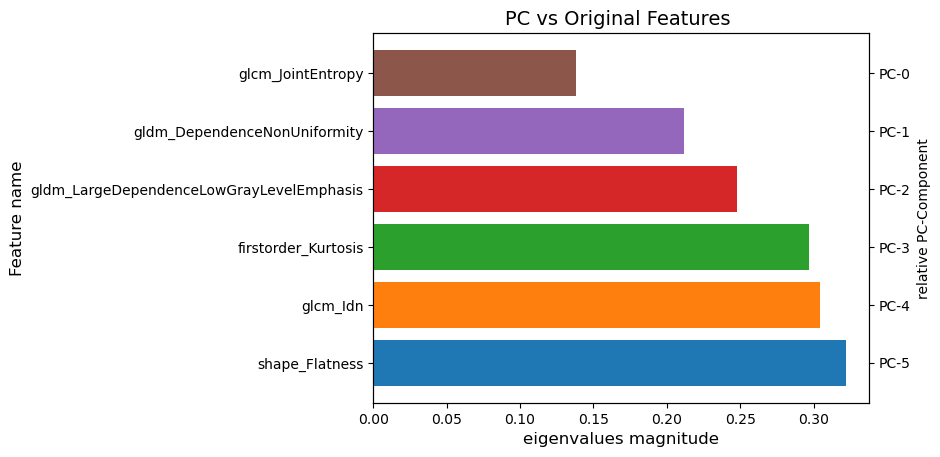
\includegraphics[width=\textwidth]{../images/importance.png}

    \caption{For each principal component (on the \textit{right}), you can see which is the original feature (on the \textit{left}) that contributes more to the relative principal component.}
    \label{importance}
    
\end{figure}


\begin{figure}[htp]

    \centering
    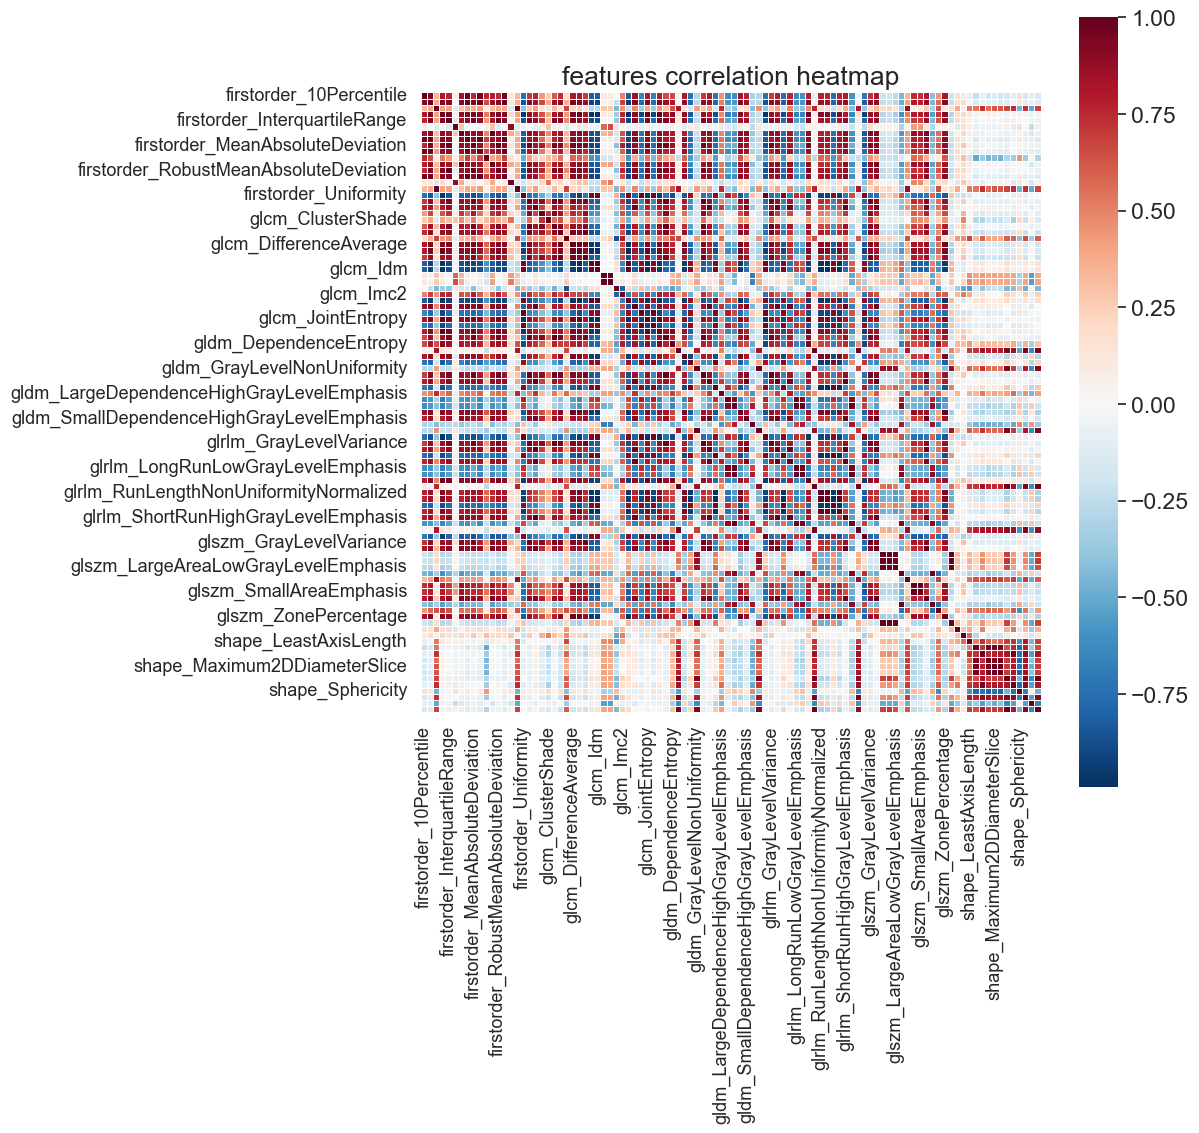
\includegraphics[width=0.9\textwidth]{../images/heatmap.png}

    \caption{Features correlation heatmap. The red color indicates a correlation, the white color indicates no correlation, and the blue color indicates anti-correlation between features. \textit{Note:} not every feature name has been plotted since 100 features caused the font size to be extremely small.}
    \label{heatmap}
    
    \end{figure}


\end{document}